% !TEX TS-program = XeLaTeX
% use the following command: 
% all document files must be coded in UTF-8
\documentclass{textolivre}
% for anonymous submission
%\documentclass[anonymous]{textolivre}
% to create HTML use 
%\documentclass{textolivre-html}
% See more information on the repository: https://github.com/leolca/textolivre

% Metadata
\begin{filecontents*}[overwrite]{article.xmpdata}
    \Title{Comparative European DigCompEdu Framework (JRC) and Common Framework for Teaching Digital Competence (INTEF) through expert judgment}
    \Author{Julio Cabero-Almenara \sep Juan Jesús Gutiérrez-Castillo \sep Antonio Palacios-Rodríguez \sep Julio Barroso-Osuna}
    \Language{en-US}
    \Keywords{teaching digital competence \sep DigCompEdu \sep evaluation \sep delphi}
    \Journaltitle{Texto Livre}
    \Journalnumber{1983-3652}
    \Volume{14}
    \Issue{1}
    \Firstpage{1}
    \Lastpage{12}
    \Doi{10.35699/1983-3652.2021.25740}

    \setRGBcolorprofile{sRGB_IEC61966-2-1_black_scaled.icc}
            {sRGB_IEC61966-2-1_black_scaled}
            {sRGB IEC61966 v2.1 with black scaling}
            {http://www.color.org}
\end{filecontents*}

\journalname{Texto Livre: Linguagem e Tecnologia}
\thevolume{14}
\thenumber{1}
\theyear{2020}
\receiveddate{\DTMdisplaydate{2020}{10}{9}{-1}} % YYYY MM DD
\accepteddate{\DTMdisplaydate{2021}{1}{4}{-1}}
\publisheddate{\DTMdisplaydate{2021}{3}{8}{-1}}
% Corresponding author
\corrauthor{Leonardo Araújo}
% DOI
\articledoi{10.35699/1983-3652.2021.25740}
% Abbreviated author list for the running footer
\runningauthor{Cabero-Almenara et al.}
\editorname{Leonardo Araújo}

\title{Comparative European DigCompEdu Framework (JRC) and Common Framework for Teaching Digital Competence (INTEF) through expert judgment}
\othertitle{Quadro Comparativo Europeu DigCompEdu (JRC) e Quadro Comum para o Ensino de Competência Digital (INTEF) por meio de opinião de especialistas}
% if there is a third language title, add here:
%\othertitle{Artikelvorlage zur Einreichung beim Texto Livre Journal}

\author[1]{Julio Cabero-Almenara \orcid{0000-XXXX-XXXX-XXXX} \thanks{Email: \url{cabero@us.es}}}
\author[1]{Juan Jesús Gutiérrez-Castillo \orcid{0000-XXXX-XXXX-XXXX} \thanks{Email: \url{jjesusgc@us.es}}}
\author[1]{Antonio Palacios-Rodríguez \orcid{} \thanks{Email: \url{aprodriguez@us.es}}}
\author[1]{Julio Barroso-Osuna \orcid{} \thanks{Email: \url{jbarroso@us.es}}}

\affil[1]{Universidad de Sevilla, España.}

\addbibresource{article.bib}
% use biber instead of bibtex
% $ biber tl-article-template

% set language of the article
\setdefaultlanguage{english}
\setotherlanguage[variant=brazilian]{portuguese}

% for spanish, use:
%\setdefaultlanguage{spanish}
%\gappto\captionsspanish{\renewcommand{\tablename}{Tabla}} % use 'Tabla' instead of 'Cuadro'

% for languages that use special fonts, you must provide the typeface that will be used
% \setotherlanguage{arabic}
% \newfontfamily\arabicfont[Script=Arabic]{Amiri}
% \newfontfamily\arabicfontsf[Script=Arabic]{Amiri}
% \newfontfamily\arabicfonttt[Script=Arabic]{Amiri}
%
% in the article, to add arabic text use: \textlang{arabic}{ ... }

% to use emoticons in your manuscript
% https://stackoverflow.com/questions/190145/how-to-insert-emoticons-in-latex/57076064
% using font Symbola, which has full support
% the font may be downloaded at:
% https://dn-works.com/ufas/
% add to preamble:
% \newfontfamily\Symbola{Symbola}
% in the text use:
% {\Symbola 😥}

\begin{document}
\maketitle

\begin{polyabstract}
\begin{abstract}
Digital technology, as one of the elements of the Knowledge Society, assumes a
determining role in educational systems, where the role of teachers is
fundamental. Along these lines, different institutions support the importance
of teaching digital skills, proposing models and conceptual frameworks. In
them, the knowledge and skills that teachers must develop are classified,
combining technological, professional, organizational and pedagogical
capacities, with different dimensions and descriptors. The objective of this
article is to compare and evaluate the feasibility of the DigCompEdu European
Digital Competence Framework for Teachers (JRC) and the Common Framework for
Teaching Digital Competence (INTEF). To do this, it is decided to carry out a
theoretical reflection on said frameworks and a subsequent Delphi study with
the coefficient of expert competence (CEC). 335 people participated, of which
275 (82.1\%) were considered experts (CEC $\geq$ 0.8). The results indicate
that, although they are very similar, the European DigCompEdu Teaching Digital
Competence Framework is the most endorsed by experts. Finally, the idea that
both are viable proposals to develop teaching digital skills through
personalized training itineraries is presented.

\keywords{teaching digital competence \sep DigCompEdu \sep evaluation \sep delphi}
\end{abstract}

\begin{portuguese}
\begin{abstract}
A tecnologia digital, como um dos elementos da Sociedade do Conhecimento,
assume um papel determinante nos sistemas educativos, onde o papel do professor
é fundamental. Nesse sentido, diferentes instituições defendem a importância do
ensino de competências digitais, propondo modelos e marcos conceituais. Neles,
classificam-se os conhecimentos e as competências que os professores devem
desenvolver, combinando capacidades tecnológicas, profissionais,
organizacionais e pedagógicas, com diferentes dimensões e descritores. O
objetivo deste artigo é comparar e avaliar a viabilidade do DigCompEdu European
Digital Competence Framework for Teachers (JRC) e do Common Framework for
Teaching Digital Competence (INTEF). Para tal, opta-se por realizar uma
reflexão teórica sobre os referidos enquadramentos e posterior estudo Delphi
com o coeficiente de competência do perito (CCP). Participaram 335 pessoas, das
quais 275 (82,1\%) foram consideradas especialistas (CCP $\geq$ 0,8). Os
resultados indicam que, embora sejam muito semelhantes, o European DigCompEdu
Teaching Digital Competence Framework é o mais endossado por especialistas. Por
fim, apresenta-se a ideia de que ambas são propostas viáveis para desenvolver o
ensino de competências digitais por meio de roteiros de treinamento
personalizados.

\keywords{ensino de competência digital \sep DigCompEdu \sep avaliação \sep Delphi}
\end{abstract}
\end{portuguese}

% if there is another abstract, insert it here using the same scheme
\end{polyabstract}


\section{Introduction}\label{sec-intro}

One of the radical transformations that has taken place in education has come
as a consequence of the strong presence that Information and Communication
Technologies are having in these institutions. But, unfortunately, this
presence has not always been accompanied, regardless of educational level, by
training plans \cite{casalOtero2018,suarezRodrguez2018,silva2019}.
As some authors have pointed out, many times they have even been given little
importance \cite{bernalBravo2019}. Other studies
affirm that even this phenomenon occurs for those who in the future would
dedicate themselves to teaching \cite{bernalBravo2019}.

The reasons pointed out by teachers for their low training do not refer to
interest in ICT, but rather as a consequence of lack of institutional support,
time, lack of resources and the non-existence of training plans
\cite{fernandezMarquez2018}. On the other hand,
when the training has been carried out, it has been carried out under models
focused more on instrumental and technological aspects than on pedagogical and
didactic dimensions \cite{semerci2018,caberoAlmenara2019a}.

This aspect leads to coining terms such as Digital Teaching Competence (DTC).
This concept does not refer exclusively to training processes focused on the
mere instrumental management of technologies. The \textcite{consejoUE2018}
points out that this is one of the key competences that citizens must
master in general and teachers specifically in the Knowledge Society.

Such is the significance that the DTC theme is acquiring, which is becoming a
consolidated line of research in the Spanish scientific context
\cite{rodrguezGarca2019}. This ranges from its description
to the search for diagnostic instruments \cite{esteve2016,duranCuartero2019,intef2017,padillaHernandez2019},
and their certification \cite{duranCuartero2019,amaya2018,gudmundsdottir2017}.

In general, the DTC can be understood as that set of knowledge, skills or
strategies of the teaching profession that allow solving the educational
problems and challenges posed by the so-called Knowledge Society \cite{prendesEspinosa2011,CaberoAlmenara2020}.
In short, as \textcite{duranCuartero2019} point out, they are a set of knowledge, skills and attitudes
necessary for a teacher to make effective use of ICT from its different
aspects, assuming pedagogical-didactic criteria for an effective integration of
the ICT in your teaching experience.

Throughout more than a decade, there have been many attempts to define
indicators, standards or models that are considered essential in the Teaching
Digital Competence \cite{CaberoAlmenara2020,caberoAlmenara2020b}.
In this article, those frameworks that can be considered the most used
at the Spanish level have been selected \cite{caberoAlmenara2019a,lazaroCantabrana2019,padillaHernandez2019,rodrguezGarca2019,silva2019,caberoAlmenara2019b}:

\begin{itemize}
\item European Framework for Teaching Digital Competence DigCompEdu \cite{redecker2017}.
\item Common Framework for Teaching Digital Competence \cite{intef2017}.
\end{itemize}


\subsection{European Framework of Digital Competence for Teaching DigCompEdu}\label{sec-euro-fram}

The European Framework for Digital Teaching Competence DigCompEdu is designed
by the Joint Research Center of the European Union or JRC \cite{redecker2017}
at the end of 2017. Its purpose is to unite European educational policies
having said framework of reference. DigCompEdu is the product of a series of
scientific studies carried out at the local, national, European and
international levels \cite{caberoAlmenara2020a,Ghomi2019,redecker2017,reisolu2020}.
Furthermore, this framework is presented as a Digital Competence
model with 6 differentiated competence areas (\Cref{fig01}).

\begin{figure}[htbp]
 \centering
 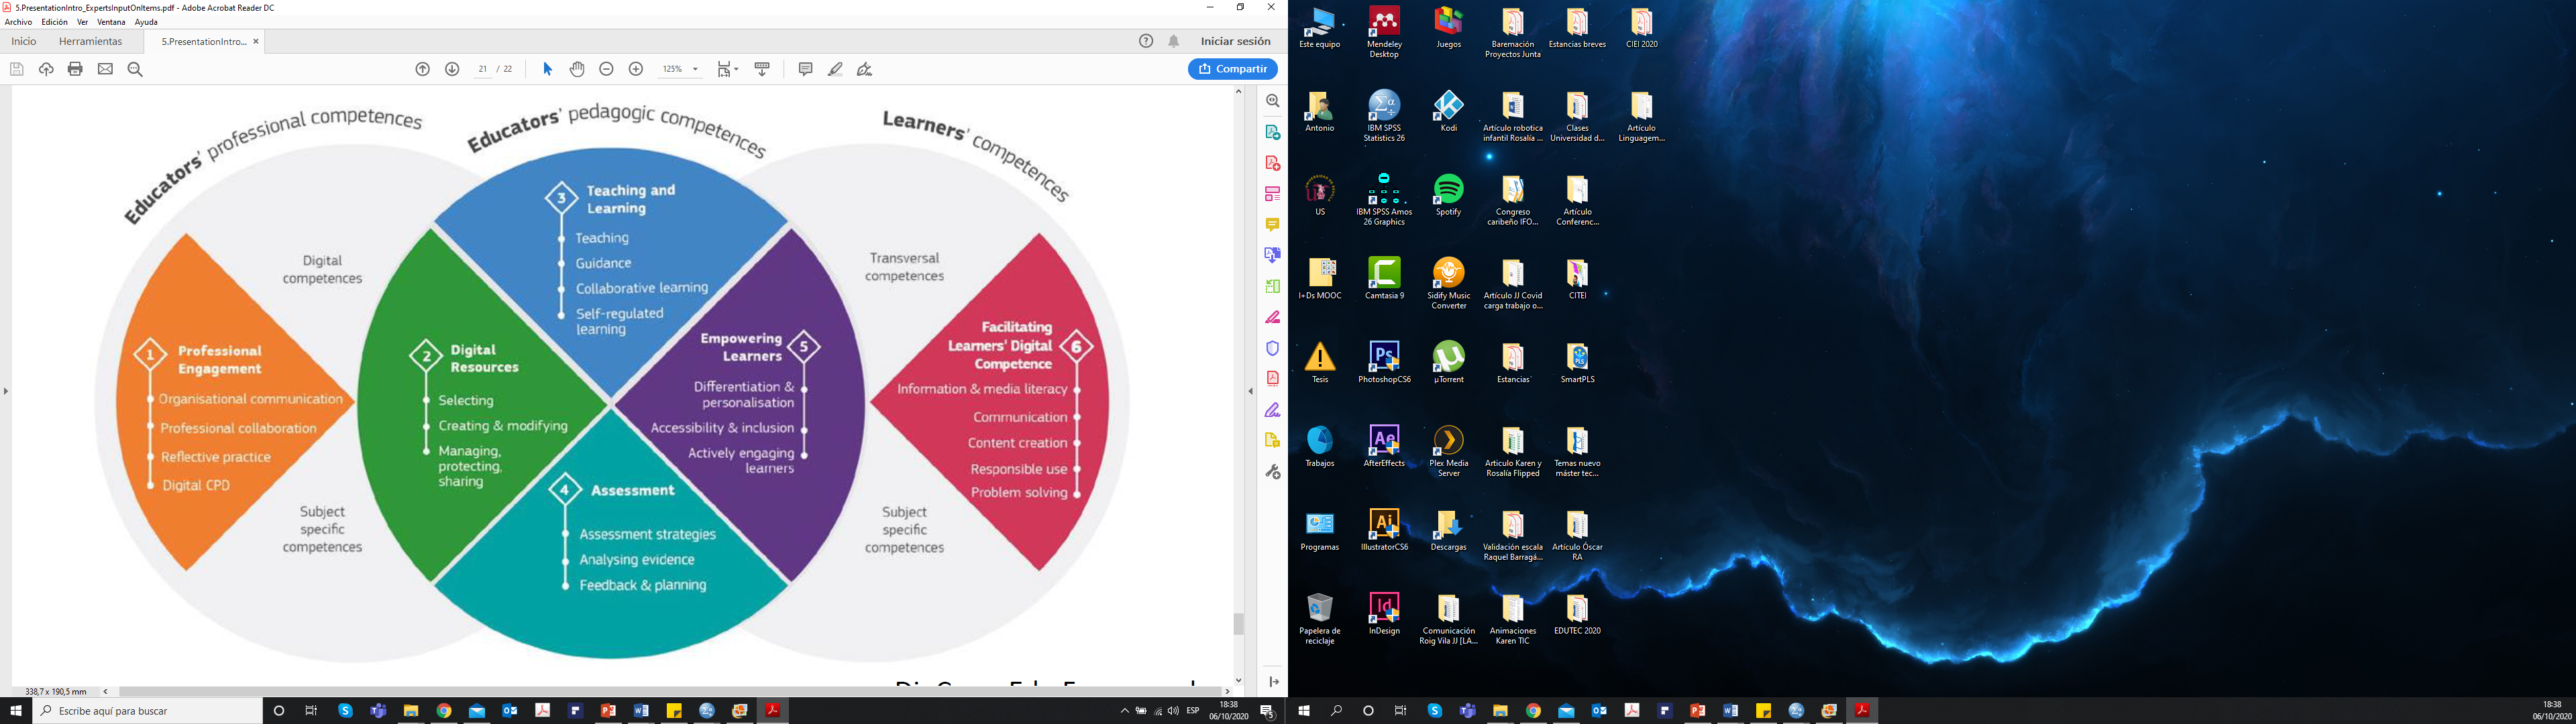
\includegraphics[width=0.75\textwidth]{fig01.png}
 \caption{DigCompEdu model.}
 \label{fig01}
 \source{JRC.}
\end{figure}

Each area is associated with a series of competencies that teachers must
possess in order to promote effective, inclusive and innovative learning
strategies, using digital tools \cite{redecker2017}. Specifically, its
areas are:

\begin{enumerate}
\item Professional engagement: focuses on teachers' work environment.
\item Digital resources: related to the sources, creation and distribution of digital resources.
\item Teaching and learning: the fundamental competence of the whole
“DigCompEdu” framework is knowing how to design, plan and implement the use of
digital technologies in the different stages of the teaching and learning
process.
\item Assesment: linked to the use of digital tools and strategies in the evaluation and improvement of teaching-learning processes.
\item Empowering learners: use of digital tools for the empowerment of students.
\item Facilitating learners´ digital competence: on how to develop and facilitate students' Digital Competence.
\end{enumerate}

In turn, DigCompEdu proposes six levels depending on the competence
qualification (\Cref{fig02}). The most basic level is called Newcomer (A1), which
would correspond to teachers with very little experience and contact with
educational technology, and the highest, Pioneer (C2), where teachers who lead
innovation with ICT would be found.

\begin{figure}[htbp]
 \centering
 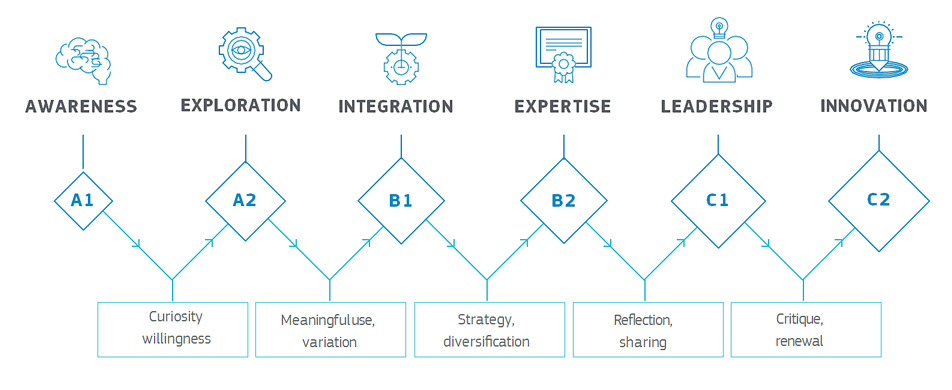
\includegraphics[width=0.85\textwidth]{fig02.jpg}
 \caption{Proficiency levels of DigCompEdu.}
 \label{fig02}
 \source{JRC.}
\end{figure}




\subsection{Common Framework for Teaching Digital Competence}\label{sec-common-fram}
The Ministry of Education, Culture and Sport of Spain launches, through the
National Institute of Educational Technologies and Teacher Training (INTEF), a
project to define the Common Framework for Digital Teaching Competence. For
this, it is based on the DigComp digital competence model, Digital Competence
for Citizenship, defined by JRC \cite{ferrari2013,vuorikari2016,intef2017}.
Like DigCompEdu, it is a generic digital
competence model for trainers, whose areas can be seen reflected in \Cref{fig03}.

\begin{figure}[htbp]
 \centering
 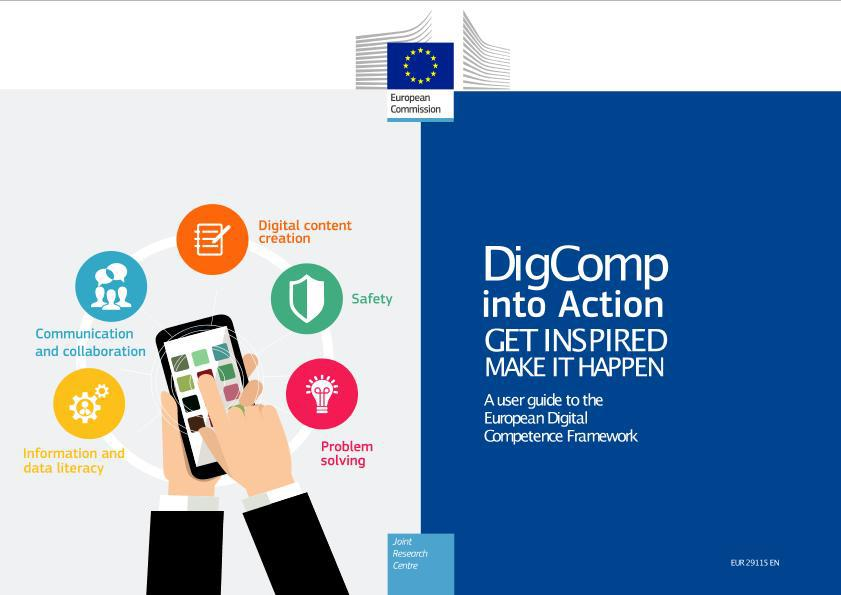
\includegraphics[width=0.65\textwidth]{fig03.jpg}
 \caption{INTEF model.}
 \label{fig03}
 \source{INTEF.}
\end{figure}


These areas can be summarized as:
\begin{enumerate}
\item Information and data literacy: identify, locate, retrieve, store, organize and analyze digital information, evaluating its purpose and relevance.
\item Communication and collaboration: communicate in digital environments,
share resources through online tools, connect and collaborate with others
through digital tools, interact and participate in communities and networks;
intercultural awareness.
\item Digital content creation: create and edit new content (texts, images,
videos \ldots), integrate and rework previous knowledge and content, make
artistic productions, multimedia content and computer programming, know how to
apply intellectual property rights and licenses use.
\item Safety: personal protection, data protection, protection of digital
identity, use of security, safe and sustainable use.
\item Problem solving: identifying needs and digital resources, making
decisions when choosing the appropriate digital tool, according to the purpose
or need, solving conceptual problems through digital means, solving technical
problems, creative use of technology, update your own competence and that of
others.
\end{enumerate}

In addition, each area is associated with a series of competencies that are developed in \Cref{fig04}.

\begin{figure}[htbp]
 \centering
 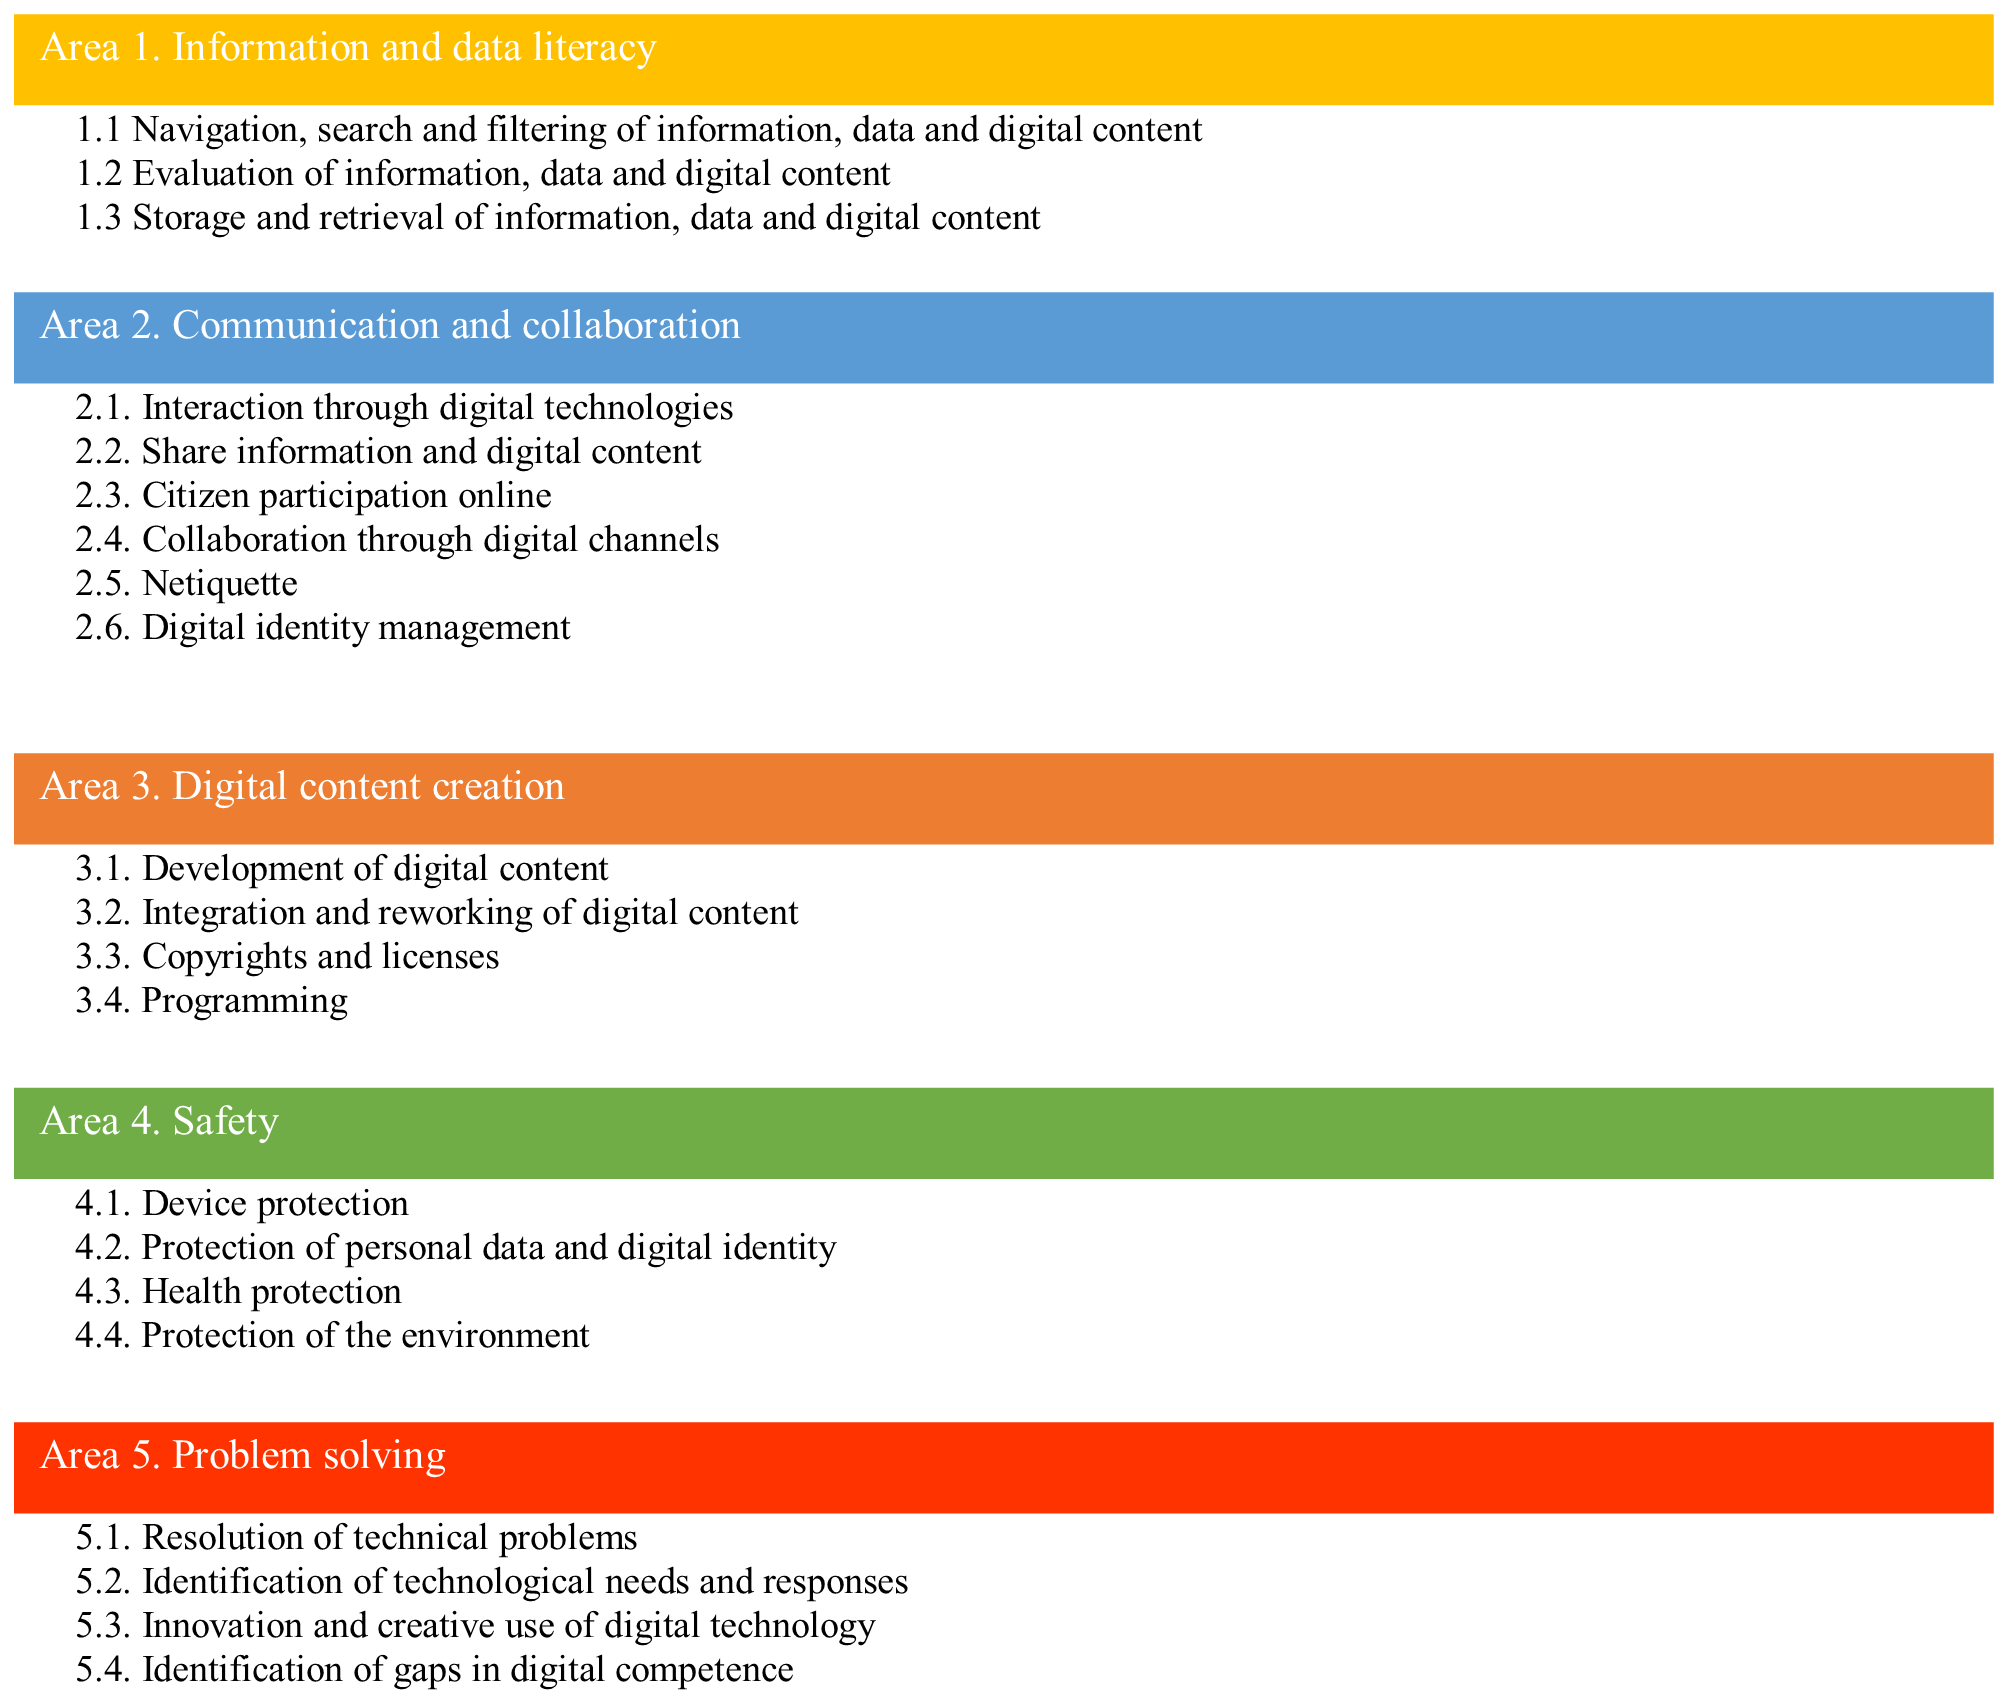
\includegraphics[width=0.8\textwidth]{fig04.png}
 \caption{Competences associated with the INTEF model.}
 \label{fig04}
 \source{INTEF.}
\end{figure}


Finally, six progressive levels of management skills are established. This
structure is designed to identify a teacher's level of digital competence. A
progressive level of development and autonomy is established that starts from
level A1 and continues up to the maximum level, C2.

Based on the comments, this article aims to compare and evaluate the DigCompEdu
European Digital Competence Framework for Teachers (JRC) and the Common
Framework for Teaching Digital Competence (INTEF).


\section{Methodology}\label{sec-meth}
This research aims to compare and evaluate the DigCompEdu European Digital
Competence Framework for Teachers (JRC) and the Common Framework for Teaching
Digital Competence (INTEF). That is, to know their differences in content and
evaluations regarding their suitability. To do this, two analysis techniques
are combined:

\begin{enumerate}
\item Comparison of the content of the competence frameworks through crossed
matrix.
\item Evaluation of the frames using Delphi design with coefficient of expert
competence (CEC) and contrast study with effect size.
\end{enumerate}


\subsection{Expert judgment}\label{sec-expert}
The expert judgment basically consists of requesting a series of people to
demand a judgment about an object, an instrument, a teaching material, or their
opinion regarding a specific aspect \cite{caberoLlorente2013}.

This strategy is increasingly widespread in educational research-evaluation
\cite{robles2015,galiciaAlarcn2017}, and specifically in the
type of studies that concern us \cite{caberoLlorente2013}. In addition, it is
closely associated with Delphi studies \cite{lopezGomez2017}. The recurring
problem with this method is that the concept of expert is quite polysemic.
Therefore, there is no unambiguous conceptualization of it that helps to
specify its defining characteristics. Therefore, the results obtained depend
directly on the quality of the experts selected for the evaluation process. For
this, there are different procedures that range from contemplating the profile
of the selected expert to other more complex ones such as the CEC \cite{caberoBarroso2013,caberoAlmenara2014,lopezGomez2017}.

In the present study, two mechanisms were established for their selection;
First, we selected them taking into account that they met the following
criteria:
\begin{itemize}
\item Teaching at Universities in the subjects of "Educational Technology",
"New Technologies applied to Education", or "Information and Communication
Technologies Applied to Education".
\item To have experience in the field of teacher training in ICT.
\item To have published an article on literacy in educational technology,
digital skills, audiovisual literacy, in Spanish and Latin American magazines,
in the last five years.
\end{itemize}

One of the problems associated with expert judgment concerns the number of
experts required for the application. Most of the proposals range between 15 -
20 experts \cite{malla1978} and 15 -35 \cite{landeta1999}. In this case,
since there were problems working with a large database and only one round of
evaluations was made, the decision is made to work with as many as possible.


\subsection{Selection and profile of experts}\label{sec-selection}
The interest in refining the selection process of the final experts is carried
out by applying the CEC \cite{caberoBarroso2013,caberoAlmenara2014,lopezGomez2017}.
This is obtained from the self-perception that the expert has
about his level of knowledge regarding the subject analyzed, as well as from
the sources that allow him to argue the decision adopted.

To obtain it, the formula is used: $K = \frac{1}{2} (Kc + Ka)$. Where $Kc$ is
the "knowledge coefficient" and $Ka$ is the argumentation coefficient.

The values used to determine the position of the expert are:
\begin{itemize}
\item $0.8 < K < 1.0$ = high competition coefficient
\item $0.5 < K < 0.8$ = mean competition coefficient
\item $K < 0.5$ = low coefficient of competition
\end{itemize}

The number of emails sent according to the criteria initially taken into
account was 747.35 responses were received. Of the total responses and, after
making the appropriate calculations, 275 experts have a $K > 0.8$, making up
the sample of this study.



\section{Resultados}
\subsection{Content analysis}
Regarding the areas, unlike the Common Framework for Teaching Digital
Competence published by INTEF which is divided into five areas, DigCompEdu is
divided into six. It is not about a differentiation only in nomenclature, but
in concepts and contents. The difference between the two frameworks is purely
conceptual, since the Spanish framework strictly focuses on the digital
competence of teaching staff, while the one published by JRC establishes other
variables more focused on the digital competence of students or educational
organizations.

Likewise, another fundamental difference between DigCompEdu and the Spanish
Teaching Digital Competence Framework is that the latter includes 21
competencies while DigCompEdu raises them to 22. However, as can be seen in the
following distribution comparison (\Cref{tab01}); Although with different
nomenclature, most of the competences published by the INTEF have been
considered in DigCompEdu.

\begin{longtable}{
    p{0.47\textwidth}
    p{0.47\textwidth}
    }
\caption{Similarities between the DigCompEdu and INTEF model.}
\label{tab01}
\\
\toprule 
DigCompEdu                      & INTEF                  \\
\midrule
6.1 Information and media literacy  & 1.1. Navigation, search and filtering of information, data and digital content \\
6.1. Information and media literacy & 1.2. Evaluation of information, data and digital content \\
6.5. Digital troubleshooting	    & 1.3. Storage and retrieval of information, data and digital content \\
1.1. Organizational communication   & 2.1. Interaction through digital technologies \\
3.2. Accompaniment & \\
5.1. Accessibility and inclusion & \\
5.2. Differentiation and customization & \\
2.3. Manage, protect and share digital resources & 2.2. Share information and digital content \\
5.3. Active students & 2.3. Online citizen participation \\
6.2. Communication and digital collaboration & \\
1.2. Professional collaboration & 2.4. Collaboration through digital channels \\
3.4. Self-regulated learning & \\
6.2. Communication and digital collaboration & \\
6.4. Responsible use & 2.5. Netiquette \\
It is not contemplated & 2.6. Digital identity management \\
6.3. Creation of digital content & 3.1. Development of digital content \\
2.2. Creation and modification of digital resources & 3.2. Integration and reworking of digital content \\
3.1. Teaching & \\
2.3. Organize, share and publish digital resources & 3.3. Copyrights and licenses \\
6.3. Digital content creation & \\
It is not contemplated & 3.4. Programming \\
6.4. Responsible use & 4.1. Device protection \\
6.4. Responsible use & 4.2. Protection of personal data and digital identity \\
6.4. Responsible use & 4.3. Health protection \\
It is not contemplated & 4.4. Protection of the environment \\
6.5. Digital troubleshooting & 5.1. Resolution of technical problems \\
5.1. Accessibility and inclusión & 5.2. Identification of technological needs and responses \\
5.2. Differentiation and customization & \\
3.4. Self-regulated learning & 5.3. Innovation and creative use of digital technology \\
5.3. Active students & \\
1.4. Continuous Digital Professional Development (CPD) & 5.4. Identification of gaps in digital competence \\
3.4. Self-regulated learning & \\
\bottomrule
\source{INTEF and JRC.}
\end{longtable}


The only competencies in the Digital Teaching Competency Framework published by
INTEF that are not mentioned in DigCompEdu are competencies 2.6., 3.4. and 4.4.

Finally, DigCompEdu establishes the same competency levels that are used in the
INTEF model, being level A1 the most basic level and C2 the most advanced.
Together, DigCompEdu assigns a role nomenclature. In the case of INTEF model,
it is not applicable since its objective is to serve as the basis for an
official certification of said competence; it is not a descriptive objective as
in the case of DigCompEdu.

\subsection{Expert judgment}
It begins by presenting the means and standard deviations achieved for each
frame, globally and in each of the dimensions (\Cref{tab02,tab03}). For a correct
interpretation of the scores, it must be taken into account that the response
scale used ranges from 1 = VN = Very negative / strongly disagree to 6 = VP =
Very positive / Strongly agree.

\begin{longtable}{
    p{0.75\textwidth}cc
    }
\caption{Expert judgment results: DigCompEdu.}
\label{tab02}
\\
\toprule
DigCompEdu model & M & SD \\
\midrule
Proffesional engagement: Ability to use digital technologies not only to improve teaching, but also to interact professionally with colleagues, students, family and different agents of the educational community. In addition, this communication through technology allows individual professional development and collective and continuous innovation in the educational organization. & 5.670 & 0.55 \\
Digital resources: Identify good educational resources. Additionally, you should be able to modify, create, and share them to suit your goals, learners, and teaching style. At the same time, you must know how to use and manage digital content responsibly, respecting copyright rules and protecting personal data. & 5.675 & 0.55 \\
Teaching and learning: Knowing how to design, plan and implement the use of digital technologies in the different stages of the teaching and learning process. In addition, a change in approaches and methodologies that are student-centered is advocated. & 5.675 & 0.58 \\
Assessment: Digital technologies can improve existing evaluation strategies and lead to new and better evaluation methods. Additionally, by analyzing the vast amount of (digital) data available on individual students' (inter-) actions, teachers can offer more specific feedback and support. & 5.520 & 0.67 \\
Empowering learners: One of the key strengths of digital technologies in education is their potential to promote the active participation of students in the learning process and their autonomy over it. In addition, digital technologies can be used to offer learning activities tailored to each student's level of competence, interests, and learning needs. However, care must be taken not to exacerbate existing inequalities (for example, in access to digital technologies) and to ensure accessibility for all students, including those with special learning needs. & 5.550 & 0.68 \\
Facilitating learners' digital competence: The ability to facilitate students' digital competence is an integral part of teachers' digital competence and is the main theme of this competence area. The response options are organized by different levels of commitment to digital technologies. & 5.655 & 0.55 \\
\midrule
TOTAL & 5.625 & 0.40 \\
\bottomrule
\source{Own elaboration.}
\end{longtable}



\begin{longtable}{
    p{0.75\textwidth}cc
    }
\caption{Expert judgment results: INTEF.}
\label{tab03}
\\
\toprule
INTEF model & M & SD \\
\midrule
Information and data literacy: Identify, locate, obtain, store, organize and analyze digital information, data and digital content, evaluating their purpose and relevance for teaching tasks. & 5.475 & 0.71 \\
Communication and collaboration: Communicate in digital environments, share resources through online tools, connect and collaborate with others through digital tools, interact and participate in communities and networks; intercultural awareness. & 5.550 & 0.67 \\
Digital content creation: Create and edit new digital content, integrate and rework previous knowledge and content, make artistic productions, multimedia content and computer programming, know how to apply intellectual property rights and licenses for use. & 5.355 & 0.85 \\
Safety: Protection of information and personal data, protection of digital identity, protection of digital content, security measures and responsible and safe use of technology. & 5.385 & 0.86 \\
Problem solving: Identify needs for the use of digital resources, make informed decisions about the most appropriate digital tools according to the purpose or need, solve conceptual problems through digital media, use technologies creatively, solve technical problems, update their own competence and the of others. & 5.465 & 0.76 \\
\midrule
TOTAL & 5.450 & 0.58 \\
\bottomrule
\source{Own elaboration.}
\end{longtable}



The analysis of the scores achieved indicates three fundamental aspects:
\begin{enumerate}
\item In both frames the mean scores are very high. This denotes the high
perceptions shown by the judges, regarding their usefulness.
\item The DigCompEdu model scores slightly higher than the INTEF model.
\item The low standard deviations indicate a strong agreement between the
diversity of the answers offered by the judges.
\end{enumerate}

Next, in order to know if there are statistically significant differences in
the assessments made by the experts on the adequacy of the frameworks, the
following hypotheses are formulated:
\begin{itemize}
\item H0 (null hypothesis): There are no significant differences between the
assessments made by the experts, with an alpha risk of 0.05.
\item H1 (alternative hypothesis): There are significant differences between
the evaluations made by the experts, with an alpha risk of 0.05.
\end{itemize}

For this, the Wilcoxon signed rank test for related samples \cite{siegel1976} is
used, as well as \textcite{cohen2013statistical} to analyze the effect size. These tests are
applied to the total assessment of both models as it is not possible to make a
comparison between areas. The results are presented in \Cref{tab04}.

\begin{table}[htpb]
\caption{Wilcoxon test and Cohen's D.}
\label{tab04}
\centering
\begin{tabular}{ll}
\toprule 
Statistical & Value \\
\midrule
W & 11027,000 \\
Standard error W & 1319,665 \\
Standardized test W & -6,023 \\
Significance W & .000 \\
Cohen's D & .351 \\
\bottomrule
\end{tabular}
\source{Own elaboration.}
\end{table}

As can be seen, the results allow rejecting H0 ($p \leq .05$). This indicates
that there are significant differences between the assessments made by the
experts. Considering the values of \textcite{cohen2013statistical}, this difference is considered
moderate.


\section{Conclusions}\label{sec-concl}
The work allows to obtain a series of conclusions. First, the similarities and
differences of the two proposed models are exposed: DigCompEdu and INTEF.
Although the general structure is very similar, DigCompEdu establishes other
variables focused on the digital competence of students or educational
organizations. Second, the different frameworks and competencies that are
incorporated within them have been positively scored by judges. This leads us
to point out that they are well-consolidated proposals and that they serve to
indicate to teachers the digital skills that they must develop to carry out
their professional activity \cite{falloon2020}. At the same time, the assessments
that different authors have made regarding the fact that the frameworks
presented are those that have the greatest significance from an international
perspective are confirmed \cite{prendesEspinosa2011,duranCuartero2019,caberoAlmenara2019a,lazaroCantabrana2019,rodrguezGarca2019,silva2019,caberoAlmenara2019b,ruizCabezas2020}.

Another of the contributions of the work also allows to point out that there
has been discrimination between the frames by the judges. In other words, the
judges value the DigCompEdu model more significantly. Such finding will serve
in the project that finances this study to approach the teacher training plan
from the perspective selected by the judges, although they must also indicate
to our institutions the guidelines on where to establish the training plans for
teachers in DTC. In any case, it is important not to confuse the results with
the fact that the INTEF model is not significant for acquiring DTC \cite{padillaHernandez2019}.
It is recalled that the results depend on
expert judges and that the INTEF model has also been scored very positively.

The study presents a series of limitations that open future lines of research
that must be considered. On the one hand, it should be noted that, although a
very conscientious process has been used for the selection of experts, there is
always doubt about the significance of their choice. Therefore, it is proposed
to carry out research of a similar nature on the specific features of teaching
in each discipline / subject: both university and non-university. The study can
also be replicated in two or three rounds, this would require less use of
experts and would require a prior commitment from them to participate in the
research in a longer time.

Finally, as a future prospect, the results of this research can be used to
guide teachers in the recognition and effective development of digital skills
for the use of ICT in training processes \cite{barraganSanchez2020}.
In addition, a possible strategy for
the development of digital skills for teachers could be consolidated according
to the assessment of the experts.


\section*{Funding}
This article is part of the project Design, production and evaluation of t-Mooc
for the acquisition by teachers of teaching digital skills
(RTI2018-097214-B-C31) funded by the Ministry of Science, Innovation and
Universities.




\printbibliography\label{sec-bib}
% if the text is not in Portuguese, it might be necessary to use the code below instead to print the correct ABNT abbreviations [s.n.], [s.l.] 
%\begin{portuguese}
%\printbibliography[title={Bibliography}]
%\end{portuguese}

\end{document}
